\documentclass[border=6pt]{standalone}
\usepackage{tikz}
\begin{document}
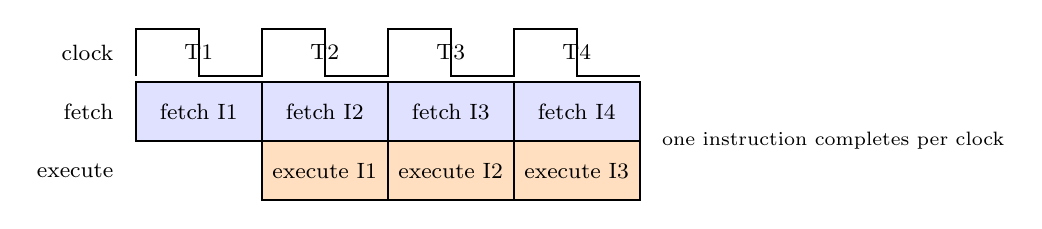
\begin{tikzpicture}[font=\small,x=1.6cm,y=0.75cm,
 F/.style={draw,thick,fill=blue!12,minimum width=1.6cm,minimum height=0.75cm,inner sep=0,font=\footnotesize},
 E/.style={draw,thick,fill=orange!25,minimum width=1.6cm,minimum height=0.75cm,inner sep=0,font=\footnotesize}]
\foreach \i in {1,...,4} \node[font=\footnotesize] at (\i-0.5,1.0) {T\i};
\draw[thick] (0,0.6) \foreach \i in {0,...,3} { -- (\i,0.6) -- (\i,1.4) -- (\i+0.5,1.4) -- (\i+0.5,0.6) } -- (4,0.6);
\node[anchor=east,font=\footnotesize] at (-0.1,1.0) {clock};
\node[anchor=east,font=\footnotesize] at (-0.1,0) {fetch};
\node[anchor=east,font=\footnotesize] at (-0.1,-1) {execute};
\foreach \i in {1,...,4} \node[F] at (\i-0.5,0) {fetch I\i};
\foreach \i in {1,...,3} \node[E] at (\i+0.5,-1) {execute I\i};
\node[font=\scriptsize,anchor=west] at (4.1,-0.5) {one instruction completes per clock};
\end{tikzpicture}
\end{document}
